%%%% CAPÍTULO 4 - RESULTADOS E DISCUSSÃO

\chapter{Resultados}\label{cap:resultados}

Este capítulo descreve os resultados preliminares do trabalho, que é um cliente \textit{web}, com foco no controle de gestão de propriedades rurais, acompanhamento de animais nas propriedades rurais e gerenciamento financeiro da propriedade, entre outras funcionalidades. 

Em seguida, será abordado o escopo, destacando as principais funcionalidades e os atores envolvidos. Em seguida, abordaremos a modelagem do sistema, que compreende a definição dos requisitos funcionais e não funcionais, juntamente com a elaboração dos diagramas de casos de uso e do modelo de entidade e relacionamento do banco de dados.

\section{Escopo do sistema}\label{sec:escopoSistema}

O cliente \textit{web} para gerenciamento de gado leiteiro será principalmente utilizado por técnicos do \gls{IDR-PR}. Sendo a principal finalidade o controle e manuseio dos dados, a fim de evitar incoerência nos registros coletados. A plataforma \textit{web} consumirá dados de uma \gls{API} \gls{REST} que está em desenvolvimento e manutenção em paralelo ao desenvolvimento deste trabalho.

Cada técnico poderá fazer o gerenciamento dos dados da propriedade vinculado, bem como dados do rebanho, dados financeiros, dados de insumos e produtos e dados de plantações.

O sistema iniciará com uma página de autenticação, caso o técnico ainda não possua cadastro ele poderá cadastrar-se. Vale ressaltar que uma propriedade pode ser relacionada a um ou mais técnicos, os técnicos só poderão analisar dados das propriedades em que estão vinculados. Estão incluídos no sistema além de cadastro e autenticação do técnico, o módulo de propriedades, módulo financeiro, módulo de animais, produtos e insumos e o módulo de plantações, sendo que exceto o módulo de propriedade, os demais são sempre referentes a uma propriedade.

No módulo dedicado às propriedades, serão cadastrados diversos dados importantes, incluindo informações sobre o produtor, colaboradores, a área destinada à bovinocultura (em hectares), coordenadas de localização e uma imagem representativa da propriedade.

Na seção voltada aos animais, serão registradas informações abrangentes, tais como dados sobre partos, inseminações, casos de mastite, doenças, medicamentos administrados, diagnósticos de prenhez, além de detalhes sobre vendas, compras e óbitos de animais.

No módulo relacionado às plantações, haverá um controle rigoroso sobre informações envolvendo pragas e doenças, abrangendo a identificação da cultura afetada, o tipo de praga ou doença identificada e o grau de infestação presente.

No que concerne ao módulo financeiro, serão meticulosamente gerenciados registros de receitas e despesas. Tais registros incluirão datas, tipos, quantidades, valores expressos em reais e descrições detalhadas, com a possibilidade de realizar agrupamentos para uma análise mais precisa.

No módulo de produtos e insumos, os usuários terão a capacidade de controlar detalhes referentes aos produtos utilizados, quantidade empregada, data de aplicação e o propósito da utilização específica.

Dessa maneira, todas as informações referentes à uma propriedade rural serão armazenadas e servirão como subsídio para que os técnicos possam auxiliar na melhora da produtividade dessas propriedades.


\section{Modelagem do sistema}\label{sec:modelagemSistema}

A modelagem do sistema inclui os diagramas e as descrições textuais para representar o problema e a solução.

Sendo assim, primeiramente esse item deve apresentar diagramas utilizados para a modelagem de negócios (ex. diagramas de atividade e estado), se esses tenham sido necessários.
Em seguida esse item deve conter a descrição dos requisitos obtidos do usuário, contendo sua respectiva classificação (funcionais e não funcionais). Sugere-se o uso de um modelo formal sugerido por autores (ex. Wazlawick, Bezerra) para a apresentação dessa classificação.

Se utilizada orientação a objetos e a UML, nesta seção ainda são apresentados, por exemplo, os diagramas de casos de uso, com suas descrições suplementares, os diagramas de classe de análise (ou modelo conceitual), de sequência e/ou comunicação, diagrama de classes de projeto.

Nesta seção também estão os diagramas da modelagem de banco de dados, como entidade-relacionamento. Nesse item pode ser apresentada a descrição de cada uma das classes do modelo de classes apresentado acima, assim como a descrição das tabelas do banco de dados. Também podem estar documentados modelos e padronizações utilizados para a interface, diagramas de navegação, a representação da arquitetura do sistema e dos padrões de projeto utilizados.

\section{Apresentação do sistema}\label{sec:apresentacaoSistema}

Apresenta as funcionalidades e o uso de recursos tecnológicos do sistema por meio de suas telas, enfatizando a interação com o sistema. A apresentação do sistema é feita sob a forma de texto, com telas e definição de padrões que forem relevantes ao contexto do trabalho. As telas são tratadas como figuras, cópias (print screen) de relatórios ou consultas também são figuras.

A \autoref{fig:cadastroPaciente} exibe a tela de acesso ao Cadastro de Pacientes.

\begin{figure}[htpb]%% Ambiente figure
  \captionsetup{width=0.43\textwidth}
  \caption{Tela de acesso ao Cadastro de Pacientes.}%% Legenda
  \label{fig:cadastroPaciente}%% Rótulo
  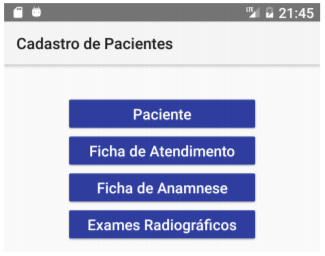
\includegraphics[scale=0.8]{cadastro-paciente}%% Dimensões e localização
  \fonte{}%% Fonte
\end{figure}

\section{Implementação do sistema}\label{sec:implementacaoSistema}

Nesta seção é documentada a implementação do sistema com partes relevantes ou exemplos de código, rotinas, funções. Inclui, ainda, a descrição técnica do uso de recursos (componentes, bibliotecas, etc.) da linguagem. Ressalta-se que cada orientador avaliará juntamente com seu orientado o que poderá ser descrito nesta seção. Isso sem que sejam revelados detalhes do sistema que possam comprometer seu uso comercial ou científico ou que a descrição fique muito sucinta ou superficial.

Em materiais e método estão quais os recursos utilizados, neste capítulo é reportado como esses recursos foram utilizados para resolver o problema.

Sugere-se colocar listagens curtas de código, enfatizando aspectos específicos das tecnologias utilizadas ou da implementação. Sugere-se, ainda, que o código não seja apresentado sob a forma de print screen, e sim copiado e colado no texto, mantendo, se possível, a formatação. Todas as listagens de código devem ser devidamente explicadas. A explicação deve ser técnica, fundamentada em aspectos conceituais e boas práticas de programação.

Enfatizar os diferenciais do sistema: procedimentos armazenados, consultas SQL, uso de componentes, uso de padrões de projeto, a forma de uso dos recursos da linguagem. Esses diferenciais são no sentido de explicitar as vantagens, desvantagens, dificuldades e facilidades que esses recursos impetraram no desenvolvimento do sistema em termos técnicos. Esses diferenciais servirão para avaliar pela utilização ou não desses recursos, pelo menos para sistemas iguais ou semelhantes ao reportado no trabalho.

Reportar a forma como o sistema foi verificado e validado. No sentido de verificar se os requisitos definidos para o mesmo foram atendidos. Os testes podem ser realizados pelo professor orientador, pelos professores que compõem a banca, por pessoas que serviram de base para as informações para o sistema e etc. Os testes podem ser realizados com base em um plano de testes elaborado juntamente com a análise e projeto do sistema. Para validar a implementação podem ser desenvolvidas rotinas de teste unitário.

Se houver implantação do sistema, mesmo que seja para teste, reportar a forma como isso foi feito, a geração de instaladores, os problemas com ambiente e sistema operacional, incluindo banco de dados e outros. Deixar explícito o procedimento para instalar e usar o sistema.

Quando for necessário, citar no texto do trabalho nomes de campos, tabelas ou rotinas específicas utilizadas na implementação de um software, utilizar a fonte courier new para destacar esses nomes.

Um exemplo de listagem de código fonte pode ser observado na \autoref{codigo:classeFoo}, que representa a classe Aluno.

\begin{sourcecode}[htb]
  \caption{\label{codigo:classeFoo}Classe Aluno}
  \begin{lstlisting}[frame=single, language=Java]
@Entity
public class Foo {
 
    @Id
    @GeneratedValue(strategy = GenerationType.IDENTITY)
    private Long id;
 
    private String nome;
    
    private Integer ra;
     
    // constructor, getters and setters
}
\end{lstlisting}
  \fonte{}
\end{sourcecode}

\section{Discussões (opcional)}\label{sec:discussoes}

O trabalho contém esta seção quando considerado que há resultados (em termos de dados) e discussões relevantes ou suficientes para justificar uma seção. Se existentes e não justificarem uma seção, eles podem estar na seção que relata a implementação do sistema.

Nesta seção estão os resultados obtidos da realização de testes quantitativos e qualitativos, independentemente da quantidade, tipo e volume de testes realizados. Os resultados dos testes são discutidos tendo como base o referencial teórico e os objetivos pretendidos com o trabalho. Esses testes podem resultar de implantação e testes de uso do sistema.
